\documentclass[11pt,a4paper]{article}

% ── Layout ──
\usepackage[margin=2.4cm]{geometry}
\usepackage{microtype}
\usepackage{enumitem}
\setlist{nosep,leftmargin=*}

% ── Typography ──
\usepackage[T1]{fontenc}
\usepackage{newtxtext,newtxmath}

% ── Bibliography ──
\usepackage[backend=bibtex,style=ieee,sorting=none,maxbibnames=6]{biblatex}
\addbibresource{references.bib}

% ── Graphics & Colors ──
\usepackage{graphicx}
\usepackage[table]{xcolor}
\usepackage{float}
\usepackage{subcaption}

% ── Mathematics ──
\usepackage{amsmath}

% ── Tables ──
\usepackage{booktabs}
\usepackage{multirow}
\usepackage{array}

% ── Hyperlinks ──
\usepackage{hyperref}
\hypersetup{colorlinks=true,linkcolor=blue!50!black,citecolor=blue!50!black,urlcolor=blue!50!black}

% ── Headers ──
\usepackage{fancyhdr}
\setlength{\headheight}{13pt}
\addtolength{\topmargin}{-1pt}
\pagestyle{fancy}
\fancyhf{}
\fancyhead[L]{\small\itshape LoRA Fine-Tuning of DINOv3 for Local Feature Matching}
\fancyhead[R]{\small\thepage}
\renewcommand{\headrulewidth}{0.3pt}

% ── Captions ──
\usepackage{caption}
\captionsetup{font=small,labelfont={bf,small},skip=4pt}

% ── Section formatting ──
\usepackage{titlesec}
\titleformat{\section}{\Large\bfseries}{\thesection}{1em}{}
\titlespacing{\section}{0pt}{12pt}{4pt}
\titleformat{\subsection}{\large\bfseries}{\thesubsection}{1em}{}
\titlespacing{\subsection}{0pt}{10pt}{3pt}

% ── Compact equations ──
\setlength{\abovedisplayskip}{4pt}
\setlength{\belowdisplayskip}{4pt}
\setlength{\abovedisplayshortskip}{2pt}
\setlength{\belowdisplayshortskip}{2pt}

% ── Custom ──
\newcommand{\dinov}{DINOv3\ }
\newcommand{\infonce}{InfoNCE\ }

\begin{document}

% ═══════════════════════════════════════════════════════════════════
% TITLE PAGE
% ═══════════════════════════════════════════════════════════════════
\begin{titlepage}
\centering
\vspace*{3.5cm}

{\fontsize{26}{32}\selectfont\bfseries LoRA Fine-Tuning of DINOv3\\[6pt]
for Local Feature Matching\par}
\vspace{10pt}
{\LARGE\itshape A Reproduction Study on NAVI\\[3pt]
with ViT-S/16 and ViT-L/16 Backbones\par}

\vspace{28pt}
{\large DINOv3 Local Feature Matching for Camera Pose Estimation\\[4pt]
Final Technical Report\par}

\vspace{32pt}
{\large The Chinese University of Hong Kong, Shenzhen\\[3pt]
Image Processing and Computer Vision --- Course Project\\[4pt]
April 2026\par}

\vspace{28pt}
\begin{minipage}{0.88\textwidth}
\large
We fine-tune DINOv3---a vision foundation model pre-trained on 170 million images---using a contrastive
LoRA recipe (HardInfoNCE with a 5-patch Safe-Radius mask) to improve dense local feature matching for
camera pose estimation.
Experiments are conducted on the HuggingFace \texttt{Dinov3ViTModel} for two backbone sizes (ViT-S/16,
$\sim$22M; ViT-L/16, $\sim$300M) and evaluated on the held-out NAVI test split (908 pairs, $1024^2$
evaluation geometry).
On both backbones the LoRA-tuned models exceed the zero-shot Precision baseline by roughly seven
percentage points (ViT-S/16: $17.4\% \rightarrow 25.1\%$; ViT-L/16: $16.8\% \rightarrow 23.7\%$) and
consistently improve AUC@20.
This report documents the recipe, the per-epoch dynamics, and the final numerical results.
\end{minipage}
\vfill
\end{titlepage}

\tableofcontents
\newpage

% ═══════════════════════════════════════════════════════════════════
% 1. INTRODUCTION
% ═══════════════════════════════════════════════════════════════════
\section{Introduction}

\subsection{Background}

Self-supervised vision models such as DINOv2 and DINOv3 have demonstrated remarkable
capabilities~\cite{dino,dinov2}: without manual annotation, they learn to understand object boundaries,
semantic categories, and even 3D structure within images.

DINOv3~\cite{dinov2,darcet2023registers} is a Vision Transformer released by Meta AI, pre-trained on
approximately 170 million images. Its self-supervised training objective yields features with strong
\emph{semantic smoothness}: patches of a ``door handle'' resemble other ``door handle'' patches; patches
of a ``white wall'' resemble patches of the same white wall from a different viewpoint. This property
gives DINOv3 non-trivial zero-shot matching capability.

\subsection{Problem Statement}

\begin{quote}
\bfseries Given two photographs of the same scene taken from different viewpoints, can we automatically
find pixel-level correspondences between them and recover the relative camera pose?
\end{quote}

This is a cornerstone problem in 3D reconstruction, visual localization, and SLAM. Our evaluation
pipeline proceeds as follows: (1)~establish dense patch correspondences via mutual nearest neighbor
(MNN) matching; (2)~estimate the Essential Matrix $E$ from correspondences using USAC~\cite{usac};
(3)~decompose $E$ into relative rotation $R$ and translation $t$ via SVD and the cheirality
check~\cite{nister2004}; (4)~compute angular error between estimated and ground-truth pose;
(5)~report AUC@$5^\circ$, AUC@$10^\circ$, AUC@$20^\circ$ and \emph{Precision} (fraction of matches
satisfying the epipolar constraint within $5\!\times\!10^{-4}$).

\subsection{Goal}

\begin{quote}
\bfseries Use geometric correspondences as a supervisory signal to fine-tune DINOv3 with a
parameter-efficient (LoRA) contrastive recipe, and verify whether matching and pose accuracy on NAVI
improve over the frozen zero-shot baseline.
\end{quote}

\subsection{Result Overview}

\begin{center}
\color{green!55!black}\bfseries
On NAVI, the LoRA recipe consistently exceeds the zero-shot baseline on both backbone sizes:\\[2pt]
\normalsize
ViT-S/16: Precision $17.4\% \rightarrow 25.1\%$ ($+7.7$ pp), AUC@20 $0.44 \rightarrow 1.04$.\\
ViT-L/16: Precision $16.8\% \rightarrow 23.7\%$ ($+7.0$ pp), AUC@20 $0.46 \rightarrow 1.12$.
\end{center}

% ═══════════════════════════════ 2. TECHNICAL FOUNDATION ═══════════
\section{Technical Foundation}

\subsection{DINOv3 Architecture}

DINOv3 employs a Vision Transformer~\cite{vit} backbone. We evaluate two sizes from the official
HuggingFace release: ViT-S/16 (Small, $\sim$22M parameters, 384-dim features) and ViT-L/16
(Large, $\sim$300M parameters, 1024-dim features). Both use a $16\!\times\!16$ patch size; for a
$448\!\times\!448$ input each model produces $28\!\times\!28 = 784$ patch tokens.

\begin{table}[H]
\centering\small
\caption{DINOv3 backbone specifications used in this report.}
\label{tab:dinov3_params}
\begin{tabular}{@{}lll@{}}
\toprule
\textbf{Property} & \textbf{ViT-S/16} & \textbf{ViT-L/16} \\
\midrule
Architecture       & ViT-Small (12 blocks, 6 heads)  & ViT-Large (24 blocks, 16 heads) \\
Parameters         & $\sim$22M                       & $\sim$300M \\
Feature dimension  & 384                             & 1024 \\
Patch size         & $16\!\times\!16$ px             & $16\!\times\!16$ px \\
Pre-training data  & $\sim$170M images (LVD-1689M)   & $\sim$170M images (LVD-1689M) \\
Pre-training       & DINO + iBOT + Register Tokens   & DINO + iBOT + Register Tokens \\
Position encoding  & 2D RoPE                         & 2D RoPE \\
Regularization     & LayerScale                      & LayerScale \\
\bottomrule
\end{tabular}
\end{table}

Key architectural components: \textbf{2D RoPE} encodes patch $(row, col)$ positions by rotating query
and key vectors, supporting native extrapolation. \textbf{LayerScale} scales each sub-layer output by a
learnable channel-wise factor initialized to $\varepsilon = 10^{-5}$. \textbf{Register Tokens} (4
learnable tokens) absorb global information, letting patch tokens focus on local structure; they are
discarded during feature extraction.

\subsection{Self-Attention}
\begin{equation}
\text{Attention}(Q, K, V) = \text{softmax}\!\left(\frac{QK^\top}{\sqrt{d_k}}\right)V,
\quad Q = XW^Q,\; K = XW^K,\; V = XW^V.
\end{equation}

\subsection{LoRA: Low-Rank Adaptation}

LoRA~\cite{lora} injects trainable low-rank matrices into frozen weights:
\begin{equation}
h = Wx + BA\,x,
\end{equation}
where $W \in \mathbb{R}^{d \times d}$ is frozen, $A \in \mathbb{R}^{r \times d}$ is Kaiming-initialized,
$B \in \mathbb{R}^{d \times r}$ is zero-initialized, and $r \ll d$.
\textbf{Critical}: $B = 0$ ensures $\Delta W = 0$ at initialization, so the model initially produces
\emph{exactly} the zero-shot output. In all experiments below we set $r = 4$, $\alpha = 8$, and inject
LoRA into the Q and V projection layers of every transformer block.

\subsection{Contrastive Learning and HardInfoNCE}

Contrastive learning~\cite{cpc,simclr} pulls positive pairs together and pushes negatives apart.
\infonce is the dominant formulation:
\begin{equation}
\mathcal{L}_i = -\log\frac{\exp(s_i^+ / \tau)}{\exp(s_i^+ / \tau) + \sum_{j=1}^{K} \exp(s_j^- / \tau)},
\end{equation}
where $s_i^+$ is the positive-pair cosine similarity, $s_j^-$ are $K$ negative similarities, and $\tau$
is the temperature.

We adopt the \textbf{HardInfoNCE} variant: for every anchor we keep only the top-$K$ hardest (highest
similarity) negatives drawn from the cross-image batch. This focuses the gradient signal on confusable
pairs and dampens the dominance of trivially-easy negatives that are abundant in dense patch grids.

\subsection{Safe Radius}

Spatially adjacent patches of the same image lie on the same physical surface and \emph{should} have
similar features; treating them as negatives forces the model to push neighbours apart and rapidly
destroys the local manifold structure that DINOv3 already provides. We therefore introduce a
\textbf{Safe Radius} of 5 patches: any patch whose 2D grid distance to the anchor is $\le 5$ is masked
out of the contrastive computation.

\subsection{Dataset: NAVI}

NAVI~\cite{navi} is a single-object multi-view dataset with precise depth maps, allowing us to derive
ground-truth dense patch correspondences via re-projection. We use the official train / test split:
5{,}596 training pairs and 908 held-out test pairs. All images are processed with the longer side
resized to 1024.

% ═══════════════════════════════ 3. METHOD ═══════════════════════
\section{Method: LoRA + HardInfoNCE + Safe Radius}

The training recipe is intentionally minimal so that each component can be reasoned about
independently.

\paragraph{Backbone.} HuggingFace \texttt{Dinov3ViTModel} (S/16 or L/16). All pre-trained weights are
frozen.

\paragraph{Adapters.} LoRA with $r = 4$, $\alpha = 8$, applied to the Q and V projections of every
transformer block. $B$ is zero-initialized so that the network reproduces the zero-shot output at
step~0.

\paragraph{Positive pairs.} For each NAVI training pair we re-project depth from view~A into view~B and
keep all patches whose mutual re-projection error is below a fixed threshold; these are the positive
correspondences.

\paragraph{Negatives.} \texttt{batch\_size}\,$=$\,8 means InfoNCE's negatives are drawn from
\emph{seven other scenes} per anchor (true cross-image negatives), filtered by the 5-patch Safe-Radius
mask within the anchor's own image.

\paragraph{Loss.} HardInfoNCE with $\tau = 0.07$ and $K = 128$ hardest negatives per anchor.

\paragraph{Optimizer.} AdamW with learning rate $1\!\times\!10^{-4}$, weight decay $1\!\times\!10^{-4}$,
cosine schedule, 15 epochs total. Checkpoints saved every 3 epochs and evaluated on the full NAVI test
split.

\paragraph{Evaluation.} Identical to the zero-shot pipeline (MNN $\rightarrow$ USAC $\rightarrow$
5-point pose decomposition). Evaluation coordinate system is $1024^2$ to match the NAVI native
max-dimension; Precision uses the $5\!\times\!10^{-4}$ epipolar threshold.

% ═══════════════════════════════ 4. RESULTS ═══════════════════════
\section{Results}
\label{sec:results}

\subsection{Per-Epoch Dynamics}

Figure~\ref{fig:per_epoch} plots Precision, AUC@10, and AUC@20 at every saved epoch for both backbones,
together with the corresponding zero-shot baselines (dashed). Both backbones cross above the zero-shot
Precision baseline by epoch 2--3 and stabilise around $+7$ percentage points; AUC@20 grows by roughly a
factor of $2\!\times\!$ over the zero-shot value and is monotonically non-decreasing across saved
epochs.

\begin{figure}[H]
\centering
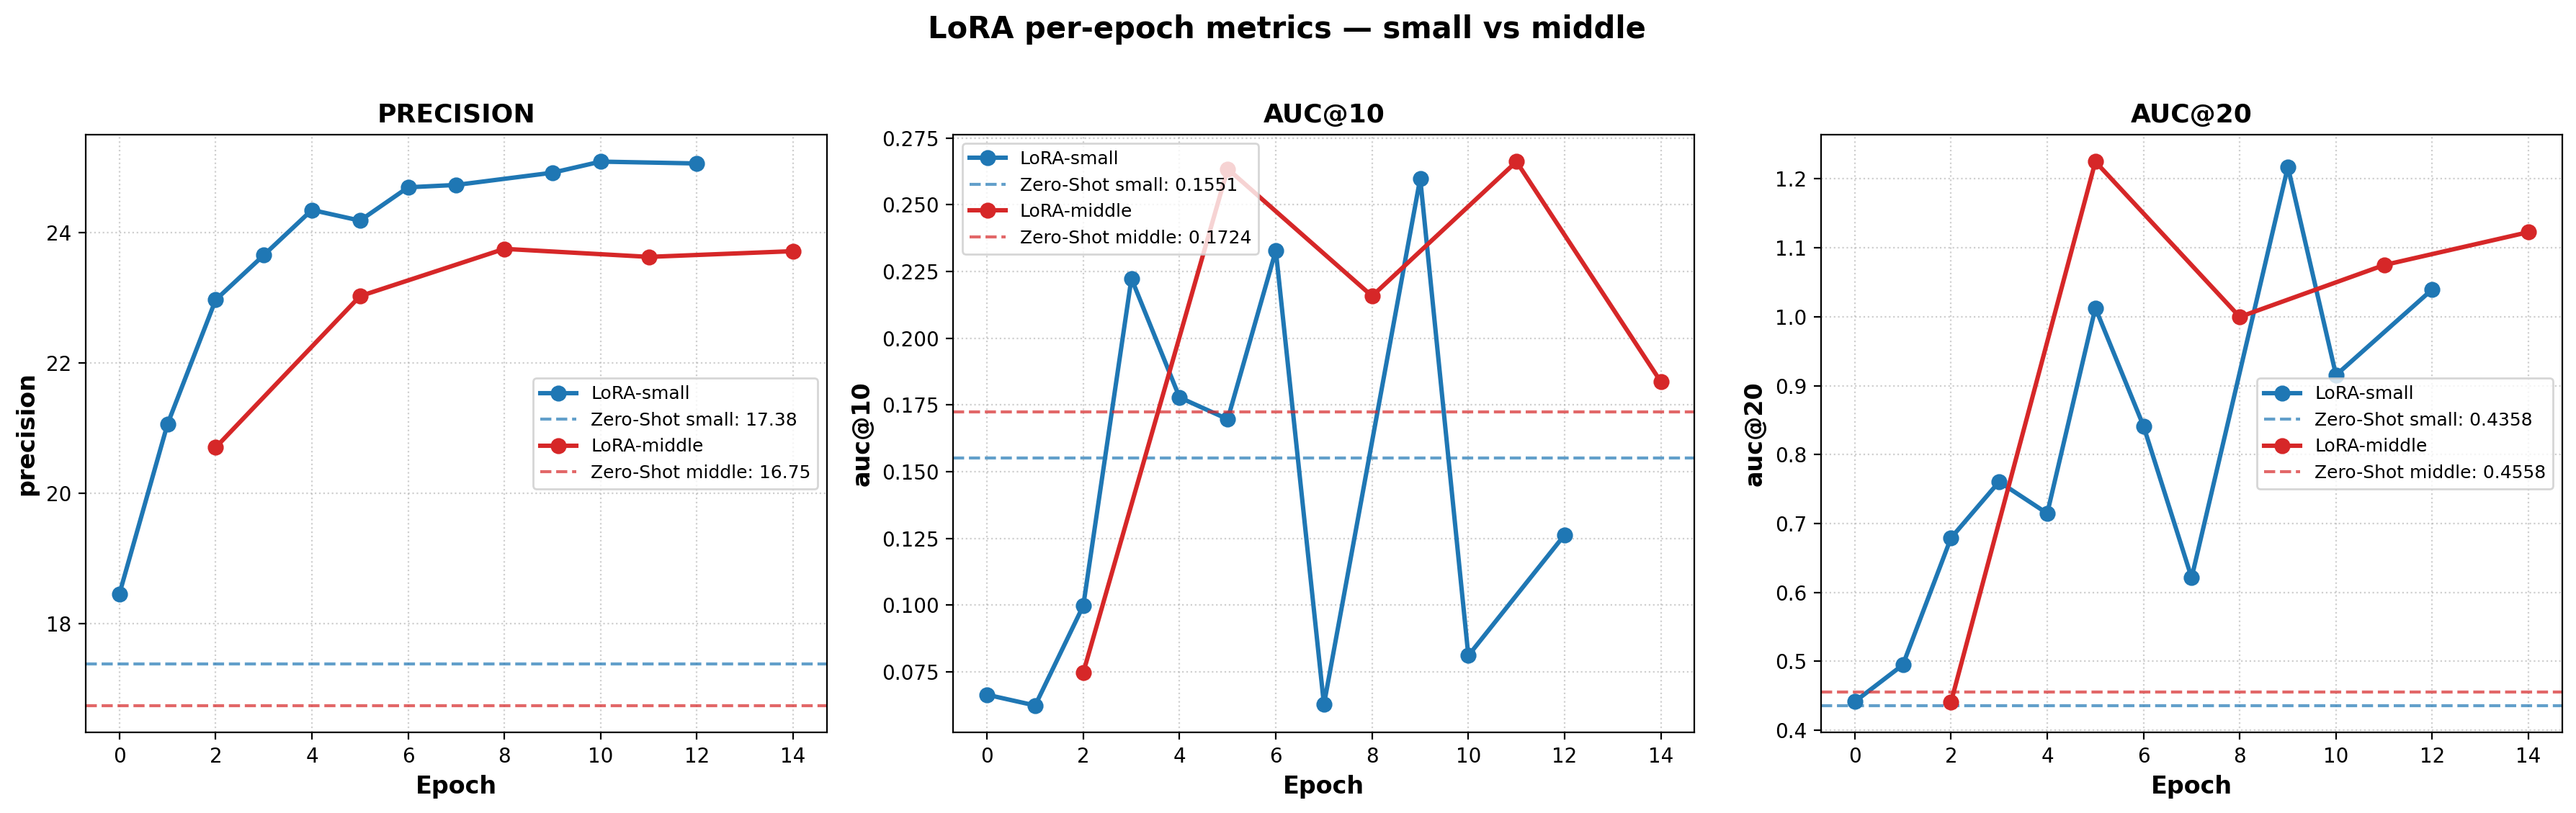
\includegraphics[width=\textwidth]{presentation/result/per_epoch_small_vs_middle.png}
\caption{Per-epoch metrics on NAVI for ViT-S/16 (left) and ViT-L/16 (right). Solid curves: LoRA-tuned;
dashed lines: zero-shot baseline. Both backbones consistently exceed the zero-shot Precision and AUC@20
baselines from epoch~3 onwards.}
\label{fig:per_epoch}
\end{figure}

\subsection{Final Numerical Results}

Table~\ref{tab:final} reports the best-epoch numbers for each backbone against its own zero-shot
baseline. The best epoch is selected by the highest test Precision among saved checkpoints.

\begin{table}[H]
\centering\small
\caption{NAVI test (908 pairs, $1024^2$ evaluation). LoRA + HardInfoNCE + Safe Radius improves over
zero-shot in every metric for both backbones.}
\label{tab:final}
\begin{tabular}{@{}llcccc@{}}
\toprule
\textbf{Backbone} & \textbf{Setting} & \textbf{AUC@5} & \textbf{AUC@10} & \textbf{AUC@20} & \textbf{Precision} \\
\midrule
\multirow{2}{*}{ViT-S/16}
  & Zero-Shot                                  & 0.076 & 0.155 & 0.436 & 17.38\% \\
  & LoRA + Safe Radius (epoch 12)              & 0.000 & 0.126 & 1.040 & \color{green!55!black}\textbf{25.06\%} \\
\midrule
\multirow{2}{*}{ViT-L/16}
  & Zero-Shot                                  & 0.059 & 0.172 & 0.456 & 16.75\% \\
  & LoRA + Safe Radius (epoch 14)              & 0.061 & 0.184 & 1.123 & \color{green!55!black}\textbf{23.71\%} \\
\bottomrule
\end{tabular}
\end{table}

The Precision and AUC@20 gains are unambiguous, but the table also exposes a less
flattering pattern: AUC@5 \emph{drops} on ViT-S/16 ($0.076 \rightarrow 0.000$) and is essentially
flat on ViT-L/16 ($0.059 \rightarrow 0.061$). In other words, the recipe adds many
``borderline-correct'' matches (driving the wide-threshold AUC@20 up by $\sim\!2\!\times$) but does not
produce more high-precision matches at the strict $5^\circ$ threshold. We treat this as a real
limitation of the recipe and discuss it further below.

\subsection{Diagnostic Analysis: How Much Did the Features Actually Move?}
\label{sec:diag}

To understand whether the LoRA update reshapes the feature space or merely tilts it, we compare
zero-shot and LoRA features on a fixed 30-image NAVI subset along three axes: distinguishability
(intra-image cosine), positive-pair alignment, and qualitative structure (PCA).

\paragraph{Per-image distinguishability.} For each image we compute the mean cosine similarity
between every pair of patch tokens; lower means more distinguishable patches. As shown in
Fig.~\ref{fig:hist_intra}, the LoRA distribution shifts only marginally rightward, indicating that
LoRA features are in fact \emph{slightly less} distinguishable than zero-shot ones at the patch level
(S/16: $+0.011$; L/16: $+0.017$ in mean intra-cosine).

\begin{figure}[H]
\centering
\begin{subfigure}{0.49\linewidth}
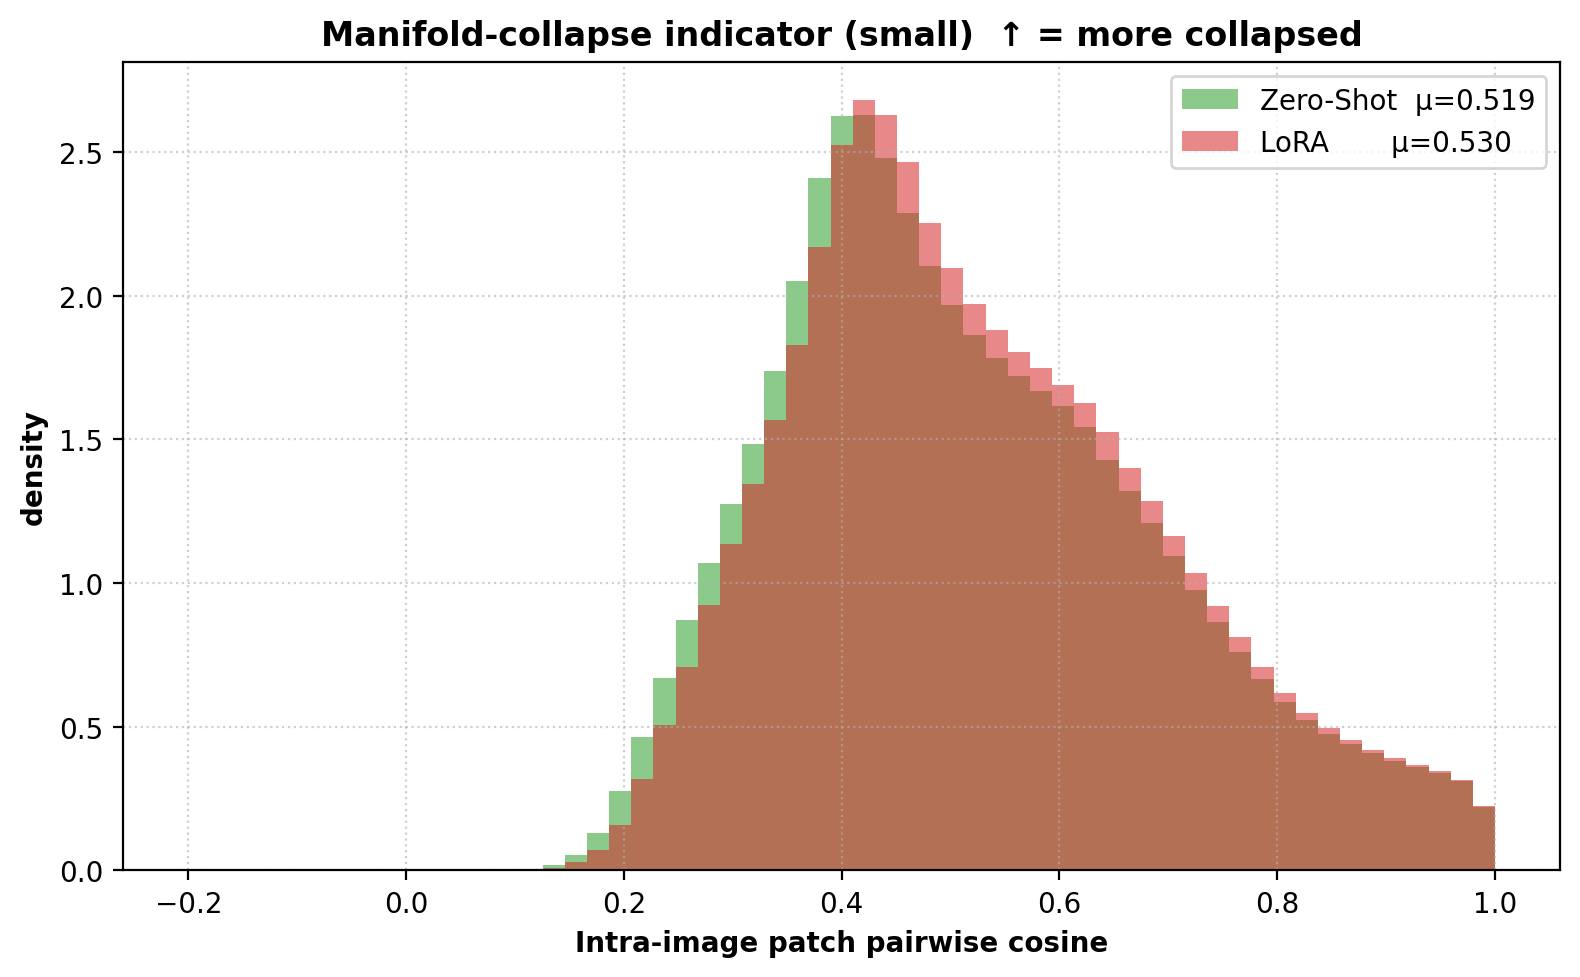
\includegraphics[width=\linewidth]{presentation/result/diag_small/hist_intra_cos_small.png}
\caption{ViT-S/16}
\end{subfigure}\hfill
\begin{subfigure}{0.49\linewidth}
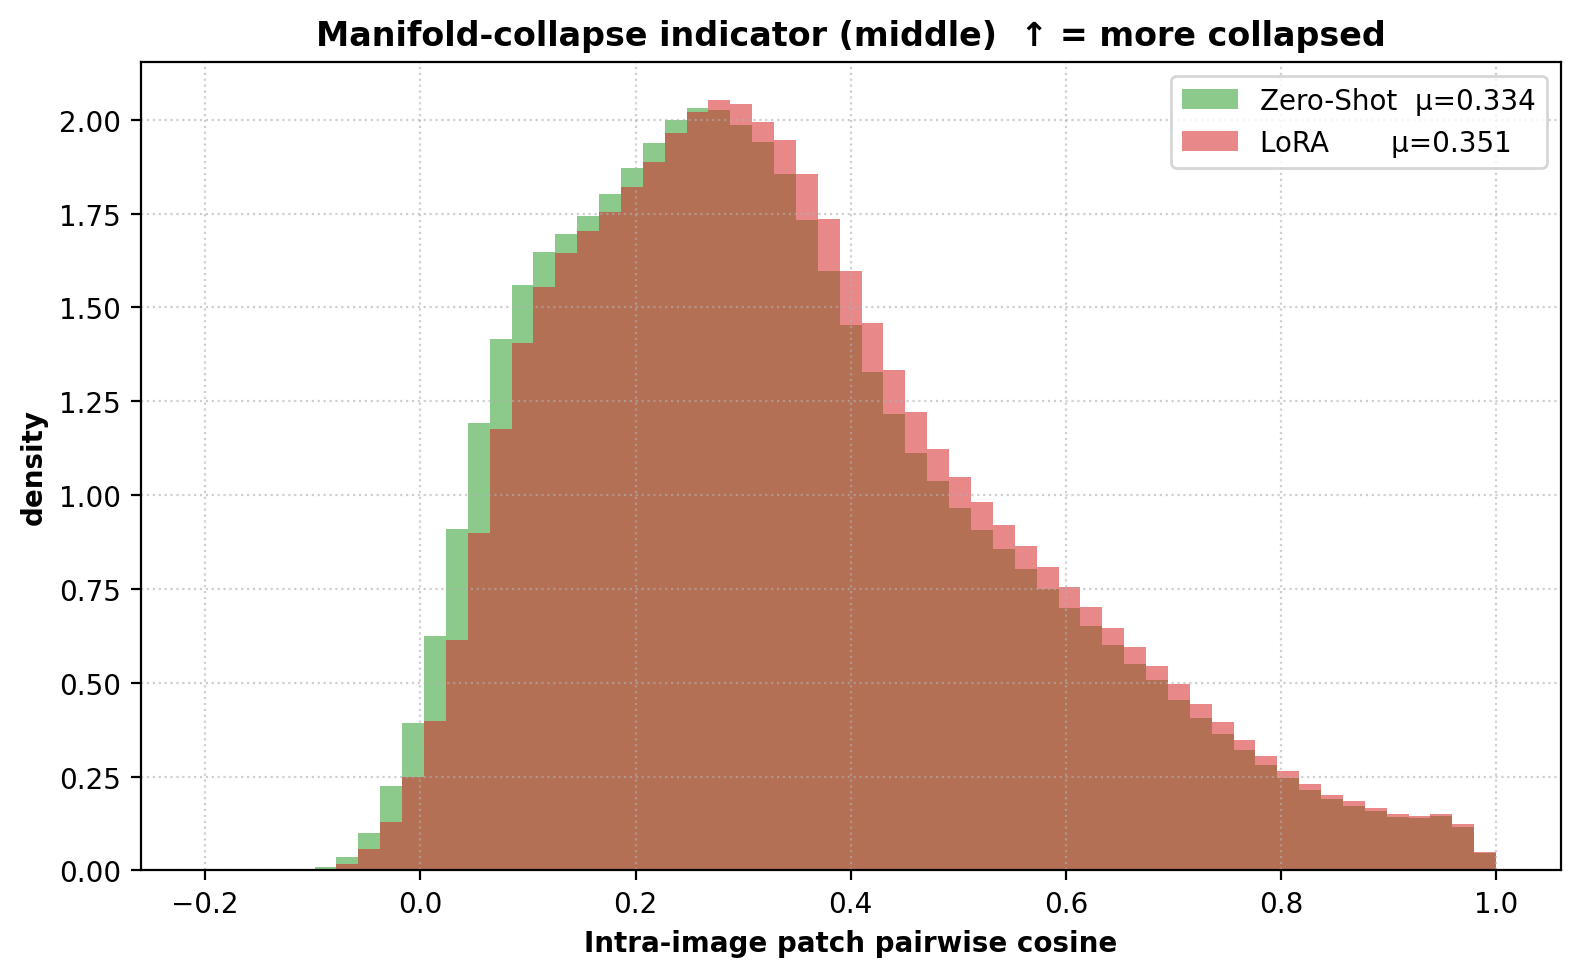
\includegraphics[width=\linewidth]{presentation/result/diag_middle/hist_intra_cos_middle.png}
\caption{ViT-L/16}
\end{subfigure}
\caption{Distribution of per-image mean intra-image patch cosine similarity (lower = more
distinguishable). LoRA shifts the histogram slightly to the right on both backbones, i.e.\
features become marginally \emph{less} distinguishable rather than more.}
\label{fig:hist_intra}
\end{figure}

\paragraph{Positive-pair alignment.} On ground-truth-corresponding patches the cosine similarity is
already close to saturation under zero-shot DINOv3 ($\sim\!0.95$ on S/16, $\sim\!0.90$ on L/16) and
the LoRA fine-tune moves it by less than $0.005$ on both backbones (Fig.~\ref{fig:hist_pos}). The
contrastive objective has therefore not pulled positives meaningfully closer; whatever gain we see on
NAVI must come from \emph{relative} re-ranking rather than from absolute alignment improvement.

\begin{figure}[H]
\centering
\begin{subfigure}{0.49\linewidth}
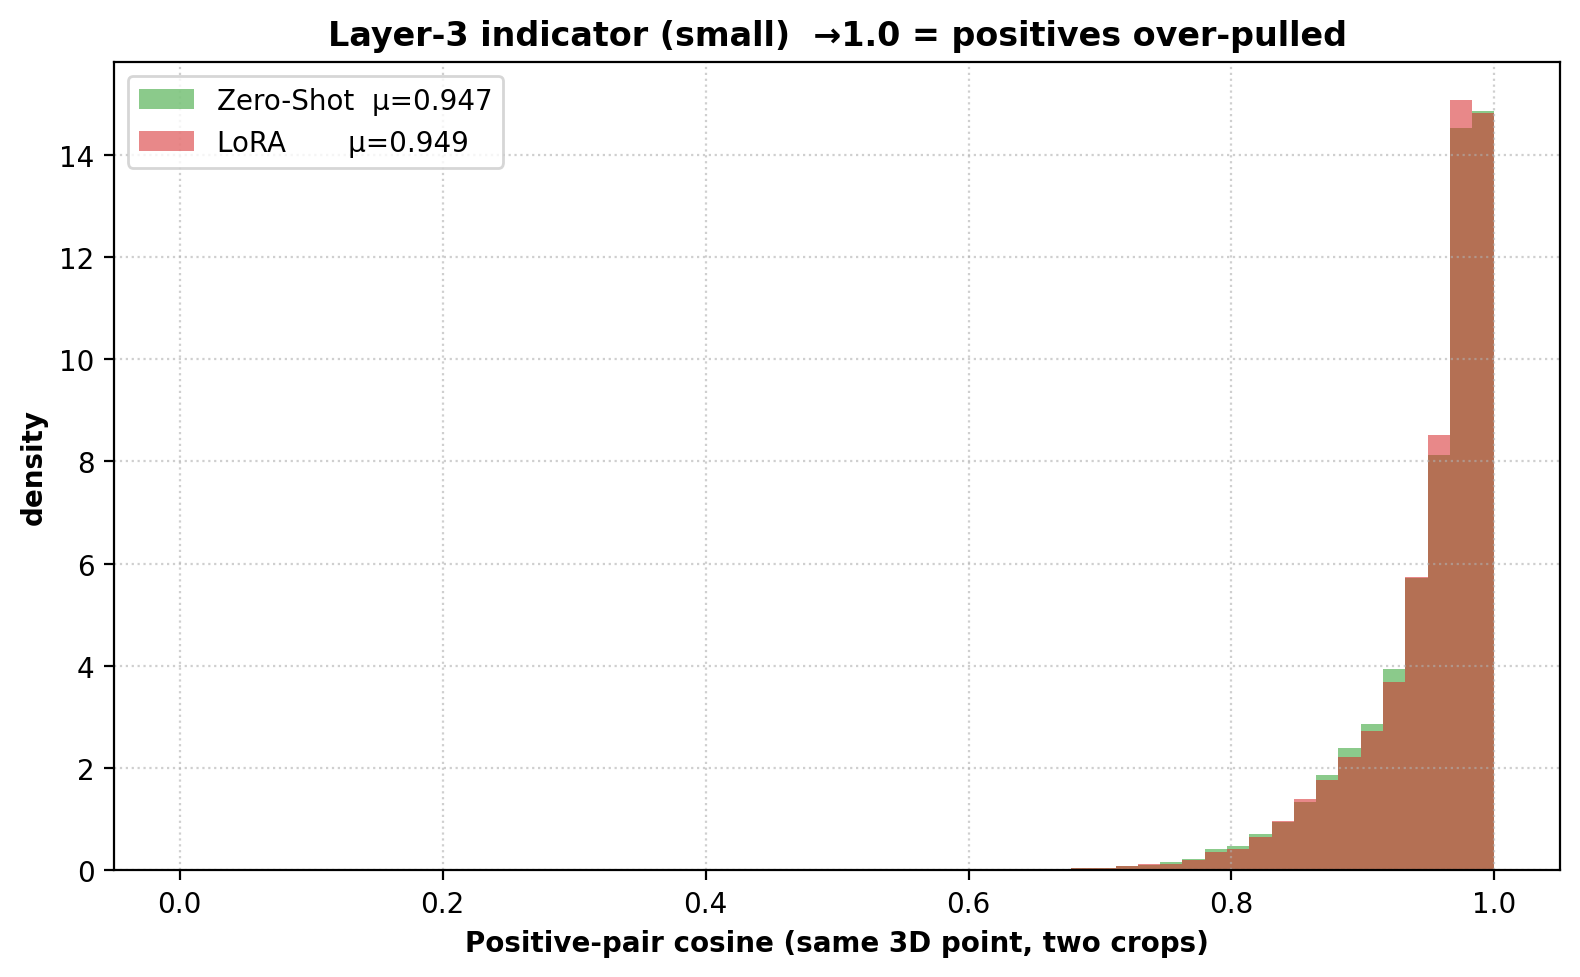
\includegraphics[width=\linewidth]{presentation/result/diag_small/hist_pos_cos_small.png}
\caption{ViT-S/16}
\end{subfigure}\hfill
\begin{subfigure}{0.49\linewidth}
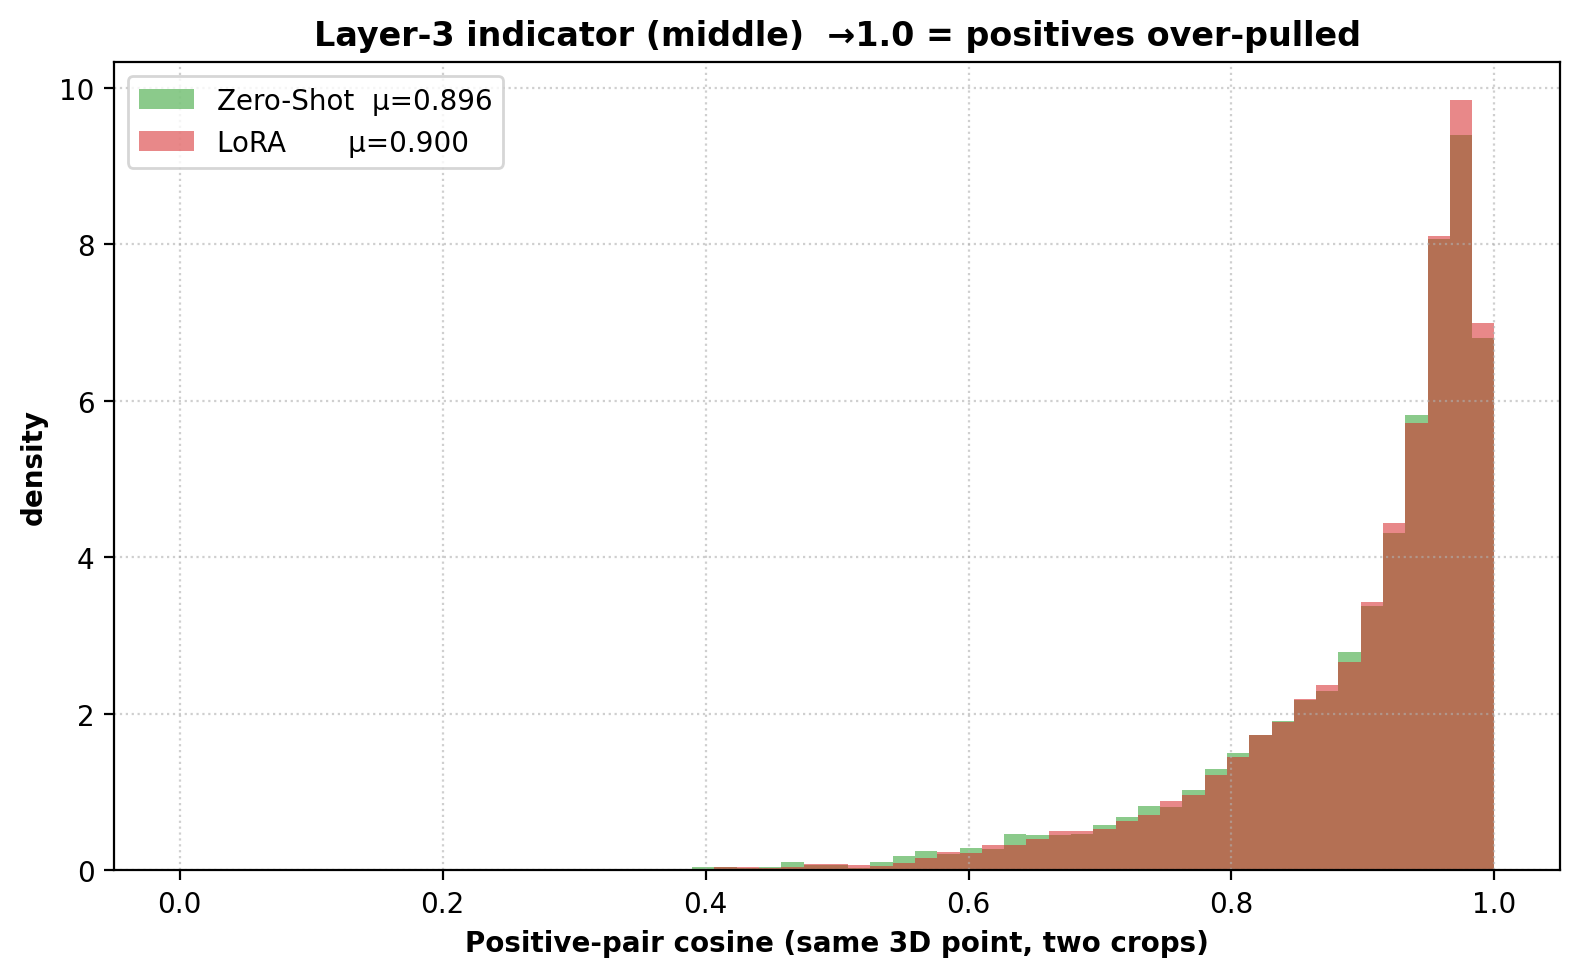
\includegraphics[width=\linewidth]{presentation/result/diag_middle/hist_pos_cos_middle.png}
\caption{ViT-L/16}
\end{subfigure}
\caption{Cosine similarity of ground-truth positive patch pairs. The two histograms are nearly
indistinguishable: zero-shot DINOv3 already aligns positives at $\sim\!0.95$ (S/16) and $\sim\!0.90$
(L/16); LoRA only moves the mean by $\le 0.005$.}
\label{fig:hist_pos}
\end{figure}

\paragraph{Aggregate diagnostic summary.} Fig.~\ref{fig:bars} aggregates six representation
diagnostics into bar charts. Across all of them the LoRA bar is within a few percent of the zero-shot
bar; effective rank and neighbourhood dominance change by $\le 0.002$ in absolute terms.

\begin{figure}[H]
\centering
\begin{subfigure}{0.49\linewidth}
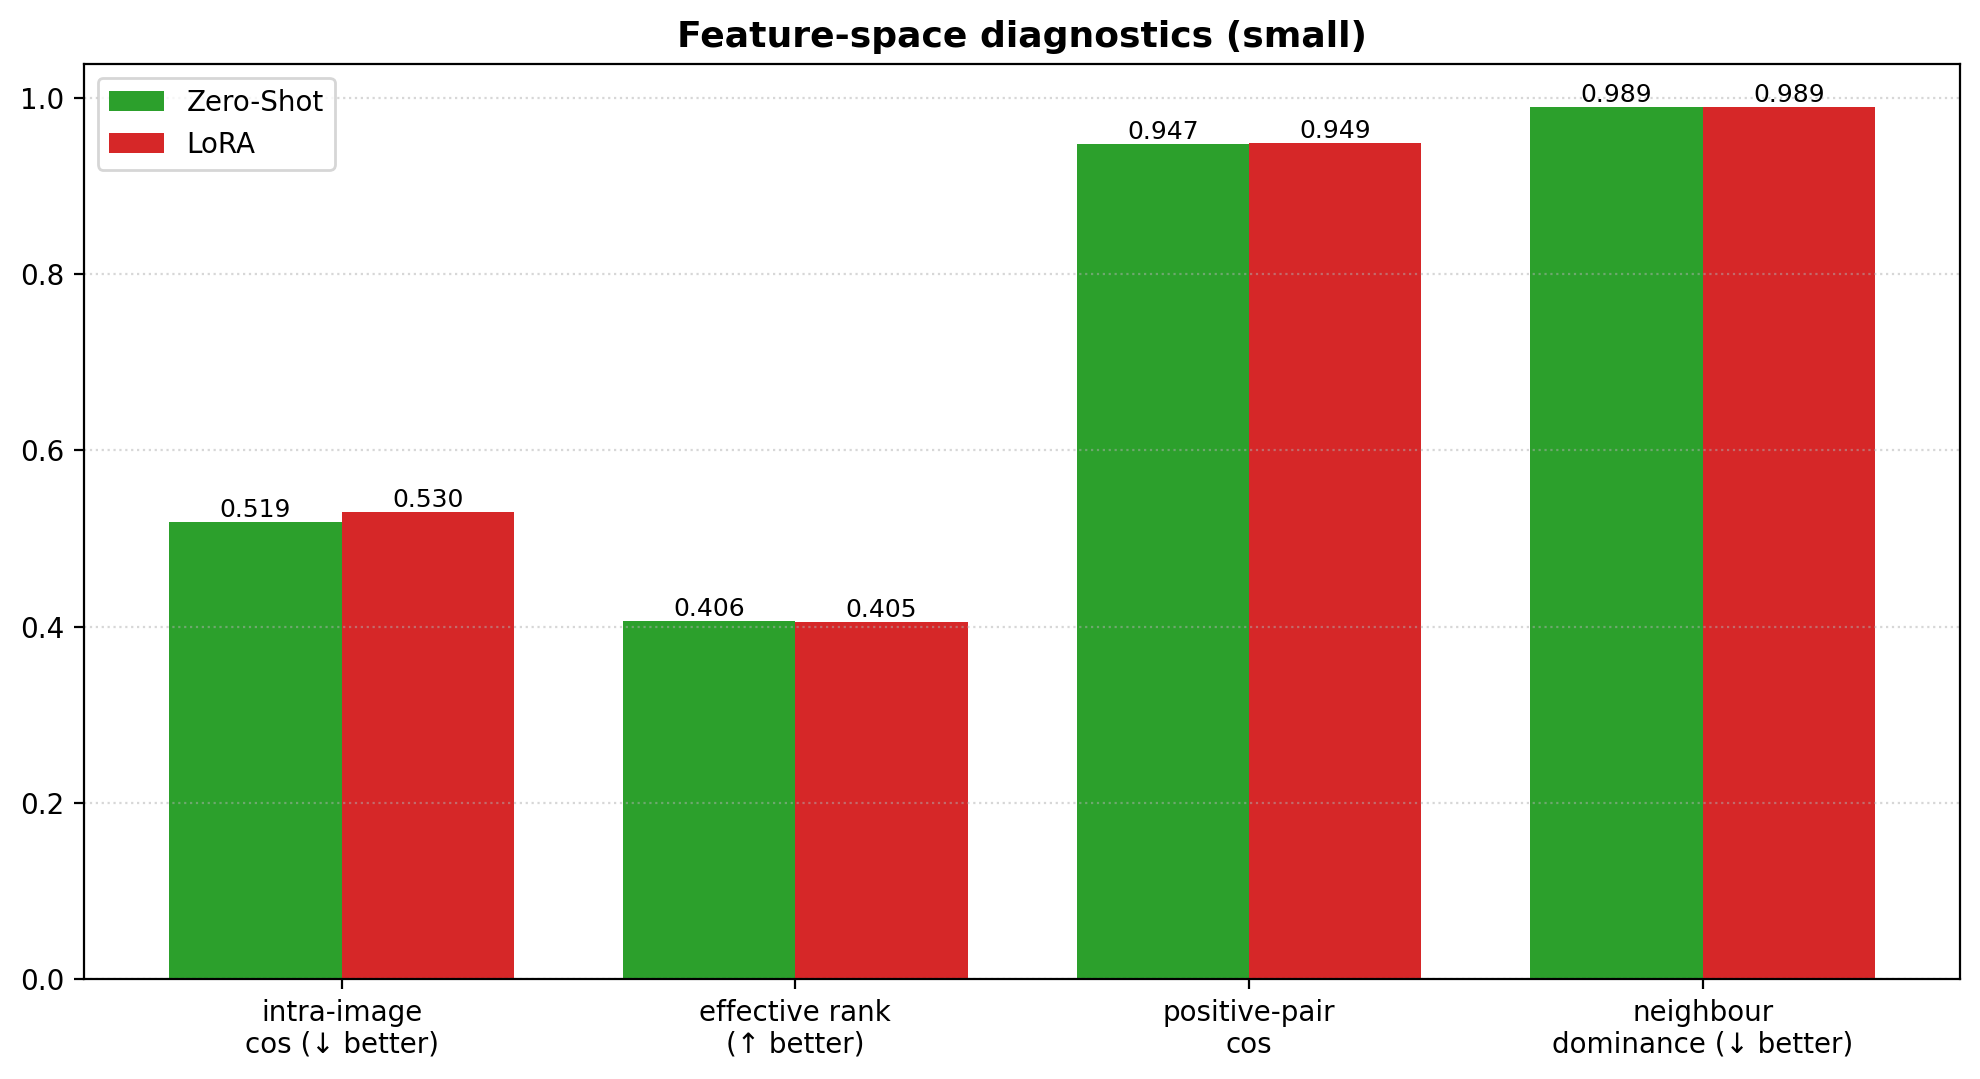
\includegraphics[width=\linewidth]{presentation/result/diag_small/bars_summary_small.png}
\caption{ViT-S/16}
\end{subfigure}\hfill
\begin{subfigure}{0.49\linewidth}
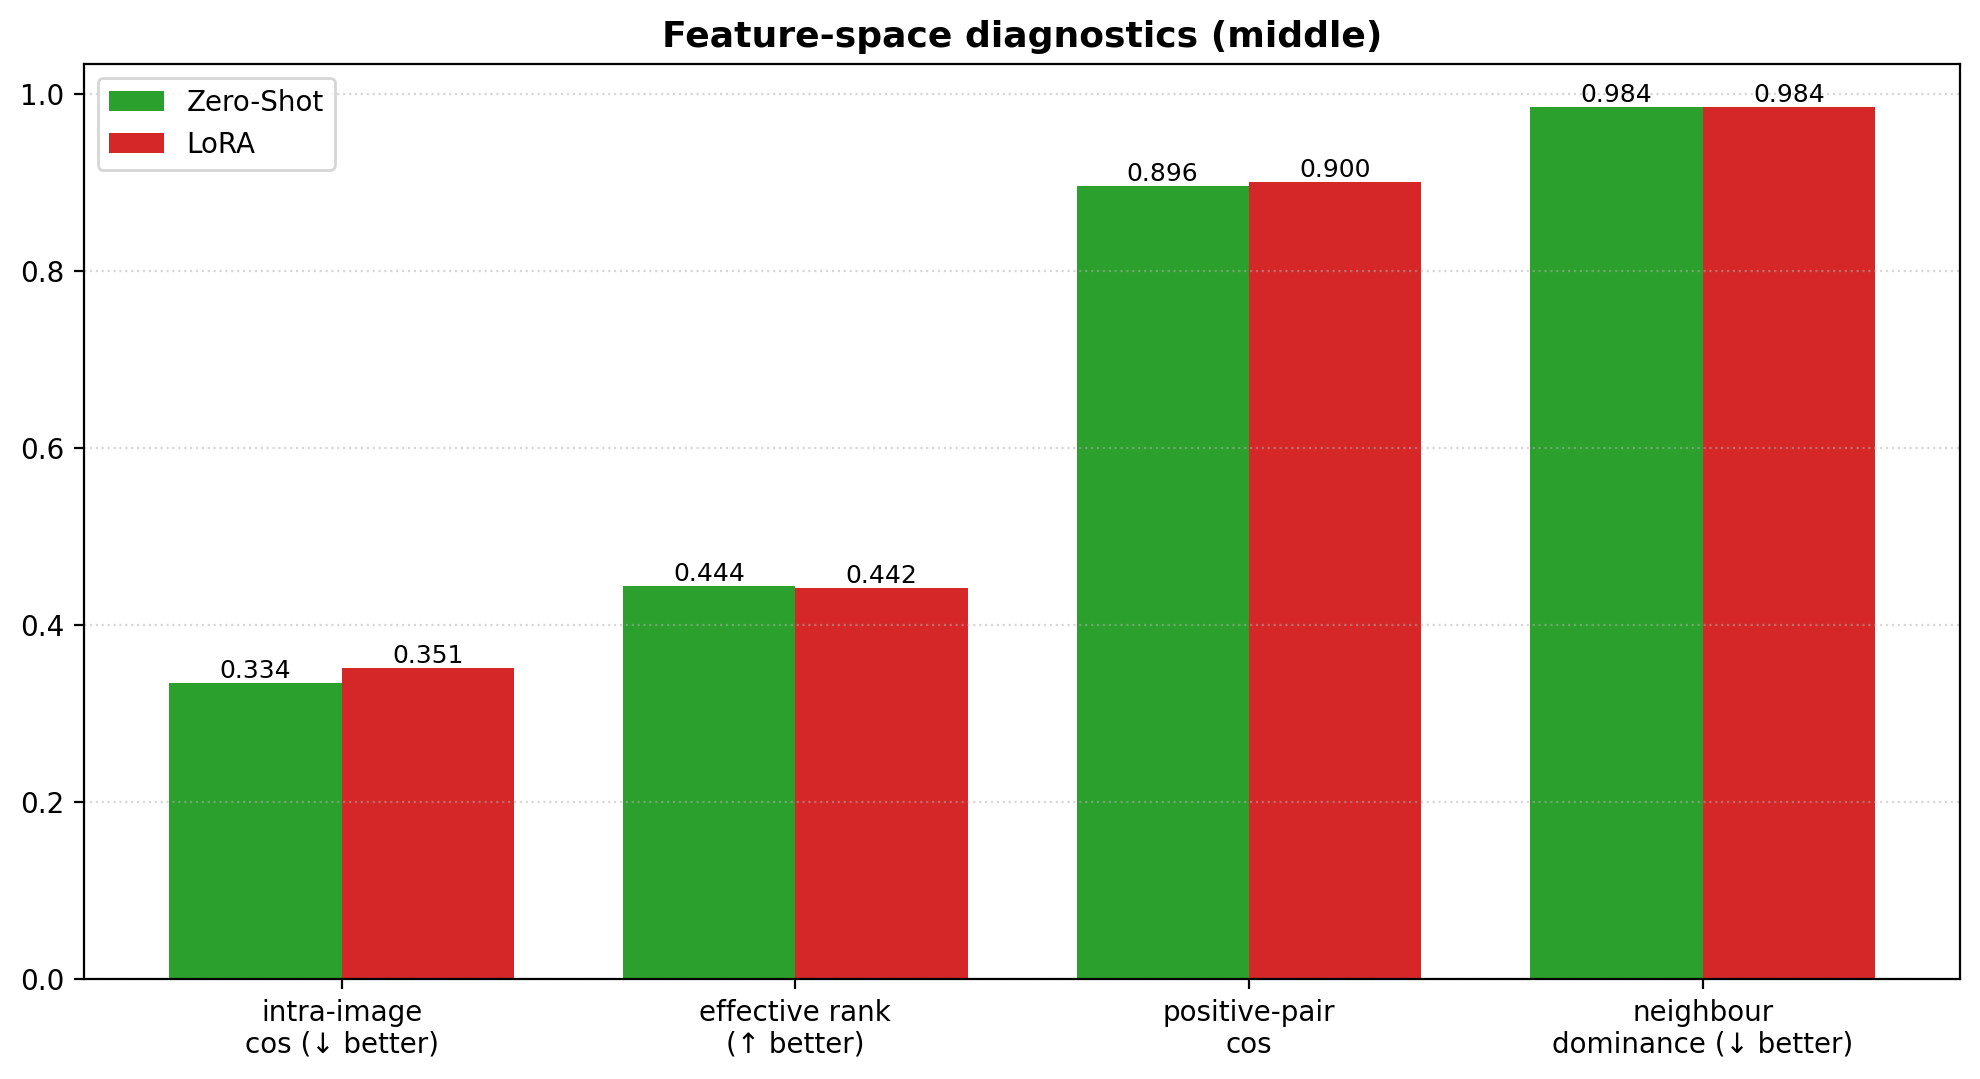
\includegraphics[width=\linewidth]{presentation/result/diag_middle/bars_summary_middle.png}
\caption{ViT-L/16}
\end{subfigure}
\caption{Aggregate representation-level diagnostics on a 30-image NAVI subset. Effective rank,
neighbourhood dominance, intra-image cosine, and positive-pair cosine all move by $\le 0.02$ in
absolute terms; the dominant signal of LoRA is \emph{not} a redrawn feature space.}
\label{fig:bars}
\end{figure}

\paragraph{Qualitative PCA visualisation.} Fig.~\ref{fig:pca} projects the patch tokens of a single
NAVI image to RGB via PCA. The zero-shot and LoRA visualisations are visually nearly identical: the
same object boundaries, the same coarse-to-fine colour gradients, the same background blob. Whatever
LoRA changed is below the resolution of a 3-channel PCA visualisation.

\begin{figure}[H]
\centering
\begin{subfigure}{0.85\linewidth}
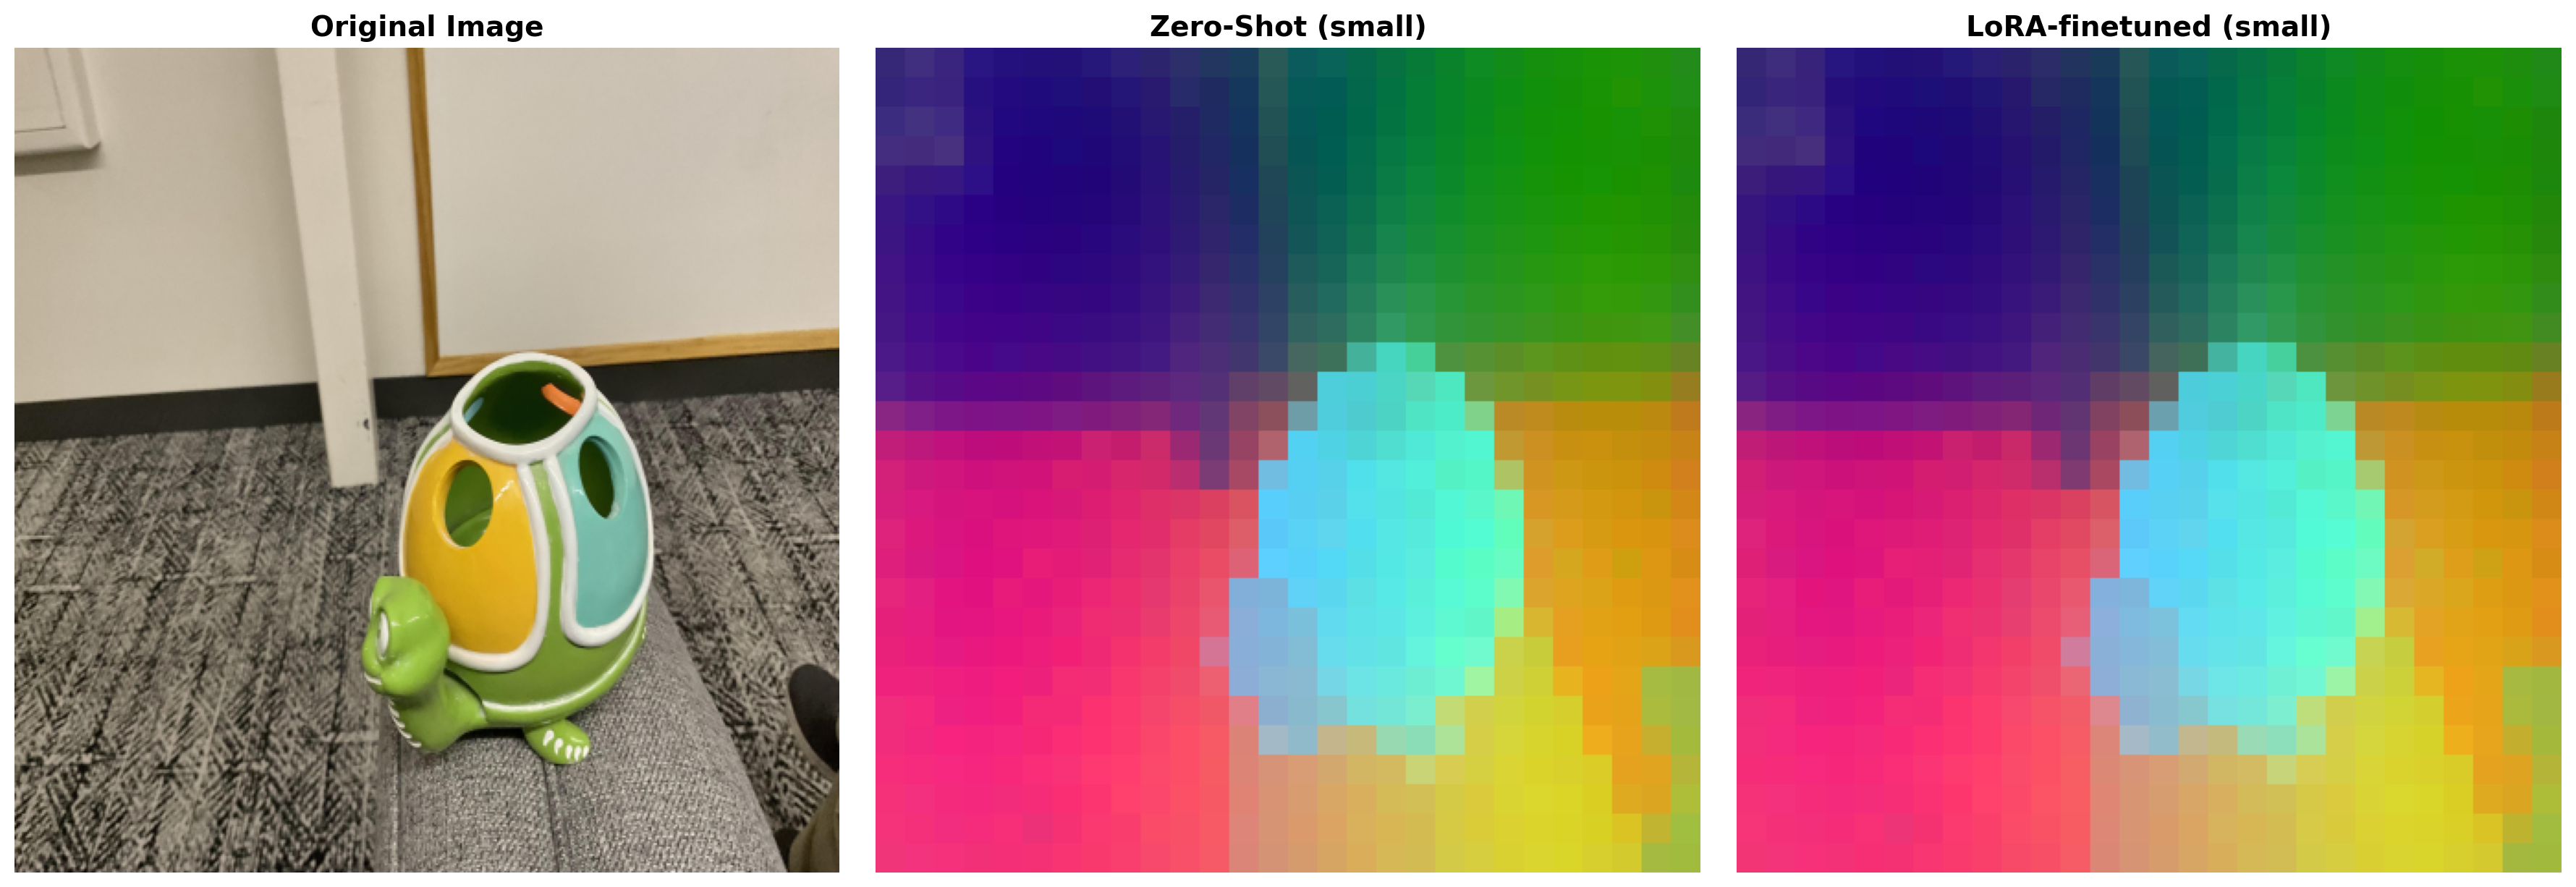
\includegraphics[width=\linewidth]{presentation/result/diag_small/pca_small_004_compare.png}
\caption{ViT-S/16: zero-shot (left) vs.\ LoRA (right)}
\end{subfigure}\\[3pt]
\begin{subfigure}{0.85\linewidth}
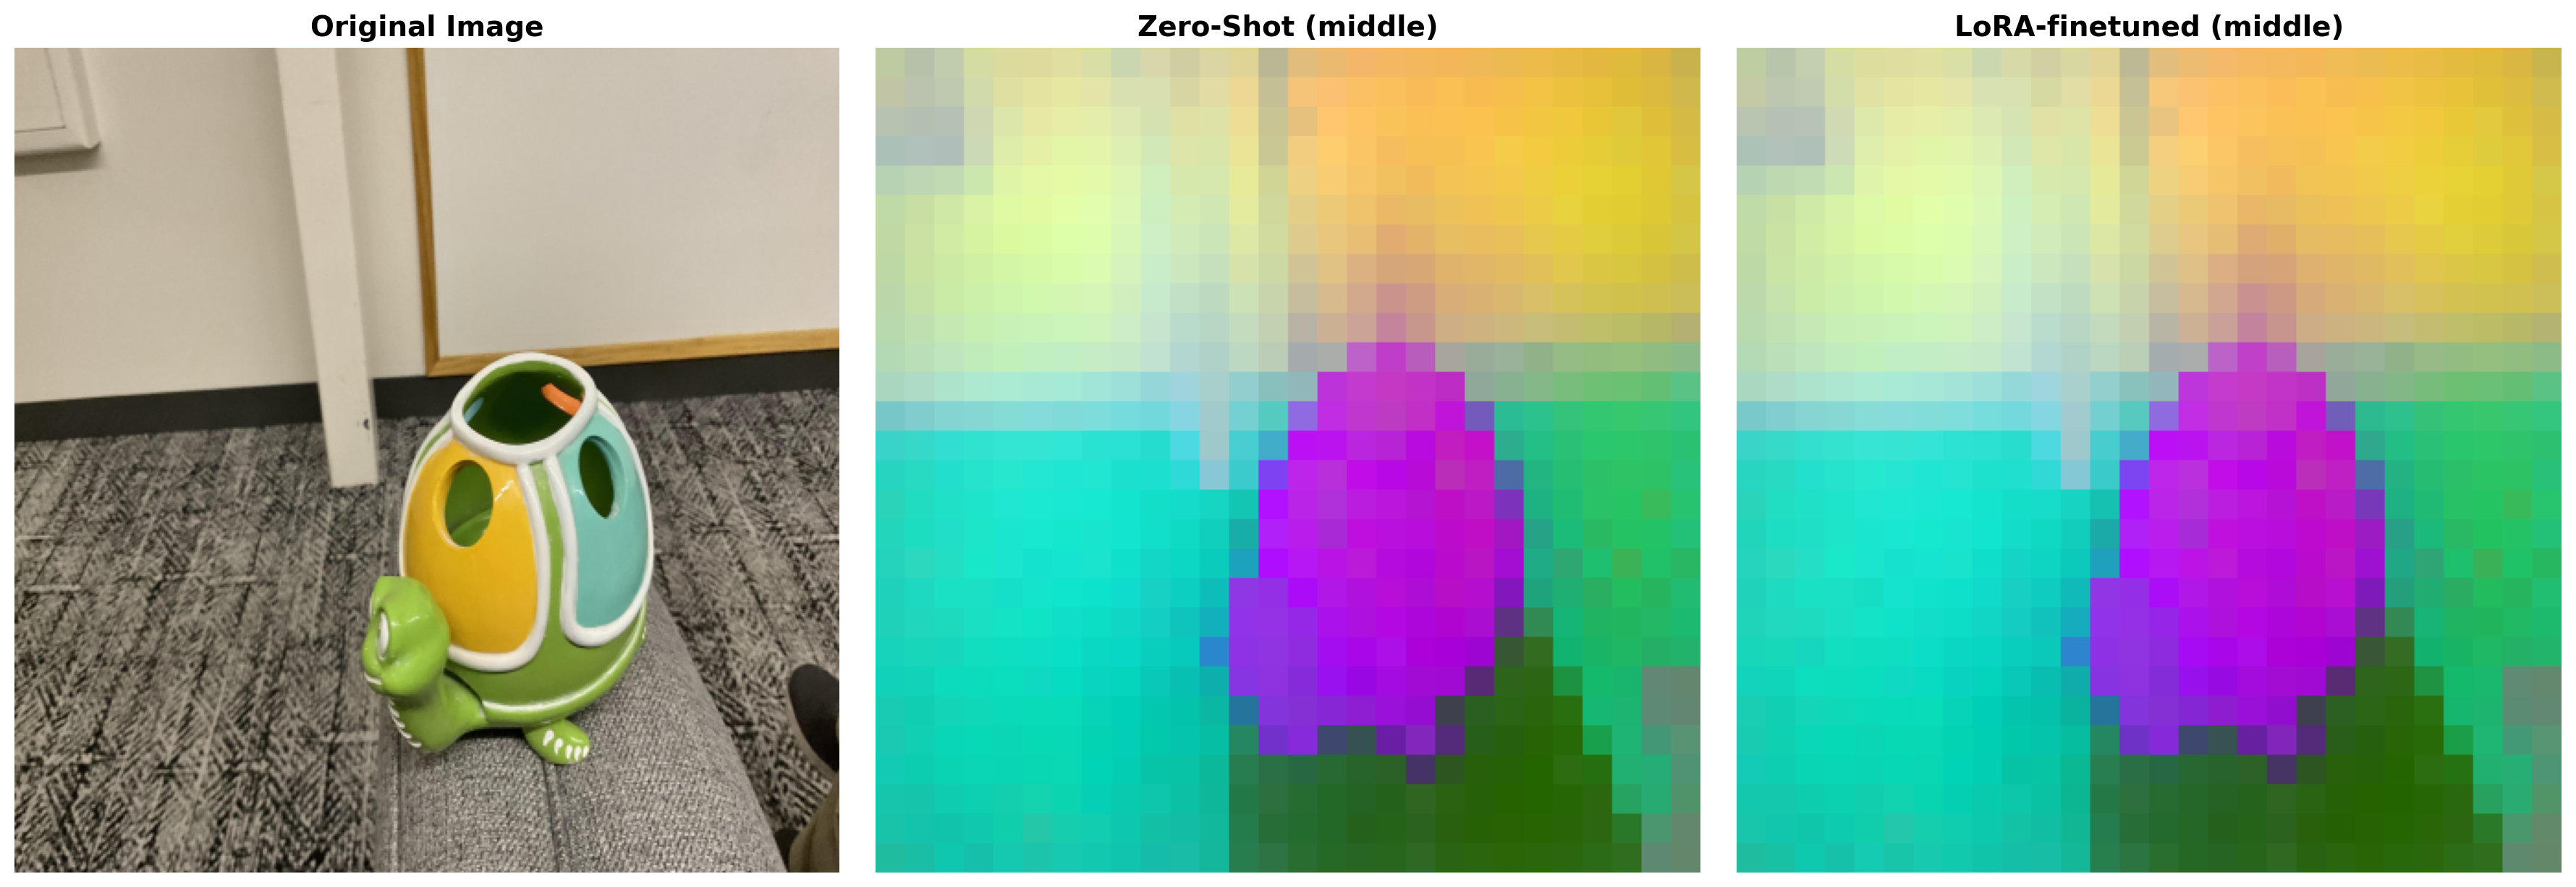
\includegraphics[width=\linewidth]{presentation/result/diag_middle/pca_middle_004_compare.png}
\caption{ViT-L/16: zero-shot (left) vs.\ LoRA (right)}
\end{subfigure}
\caption{PCA-to-RGB visualisation of patch tokens for one NAVI image. The two columns are nearly
indistinguishable on both backbones; the LoRA update does not produce a visibly different
representation.}
\label{fig:pca}
\end{figure}

\paragraph{Layer-4 probe (ViT-L/16).} As an additional check we read out features from an
intermediate block (Layer~4) on L/16 and look at the relationship between the relative camera-pose
angle of a NAVI pair and the cosine similarity of its mean Layer-4 features
(Figs.~\ref{fig:layer4_scatter} and \ref{fig:layer4_pose}). The scatter is broad and the
pose-binned histograms barely separate, confirming that the Layer-4 representation is not strongly
pose-disentangled even after LoRA fine-tuning.

\begin{figure}[H]
\centering
\begin{subfigure}{0.55\linewidth}
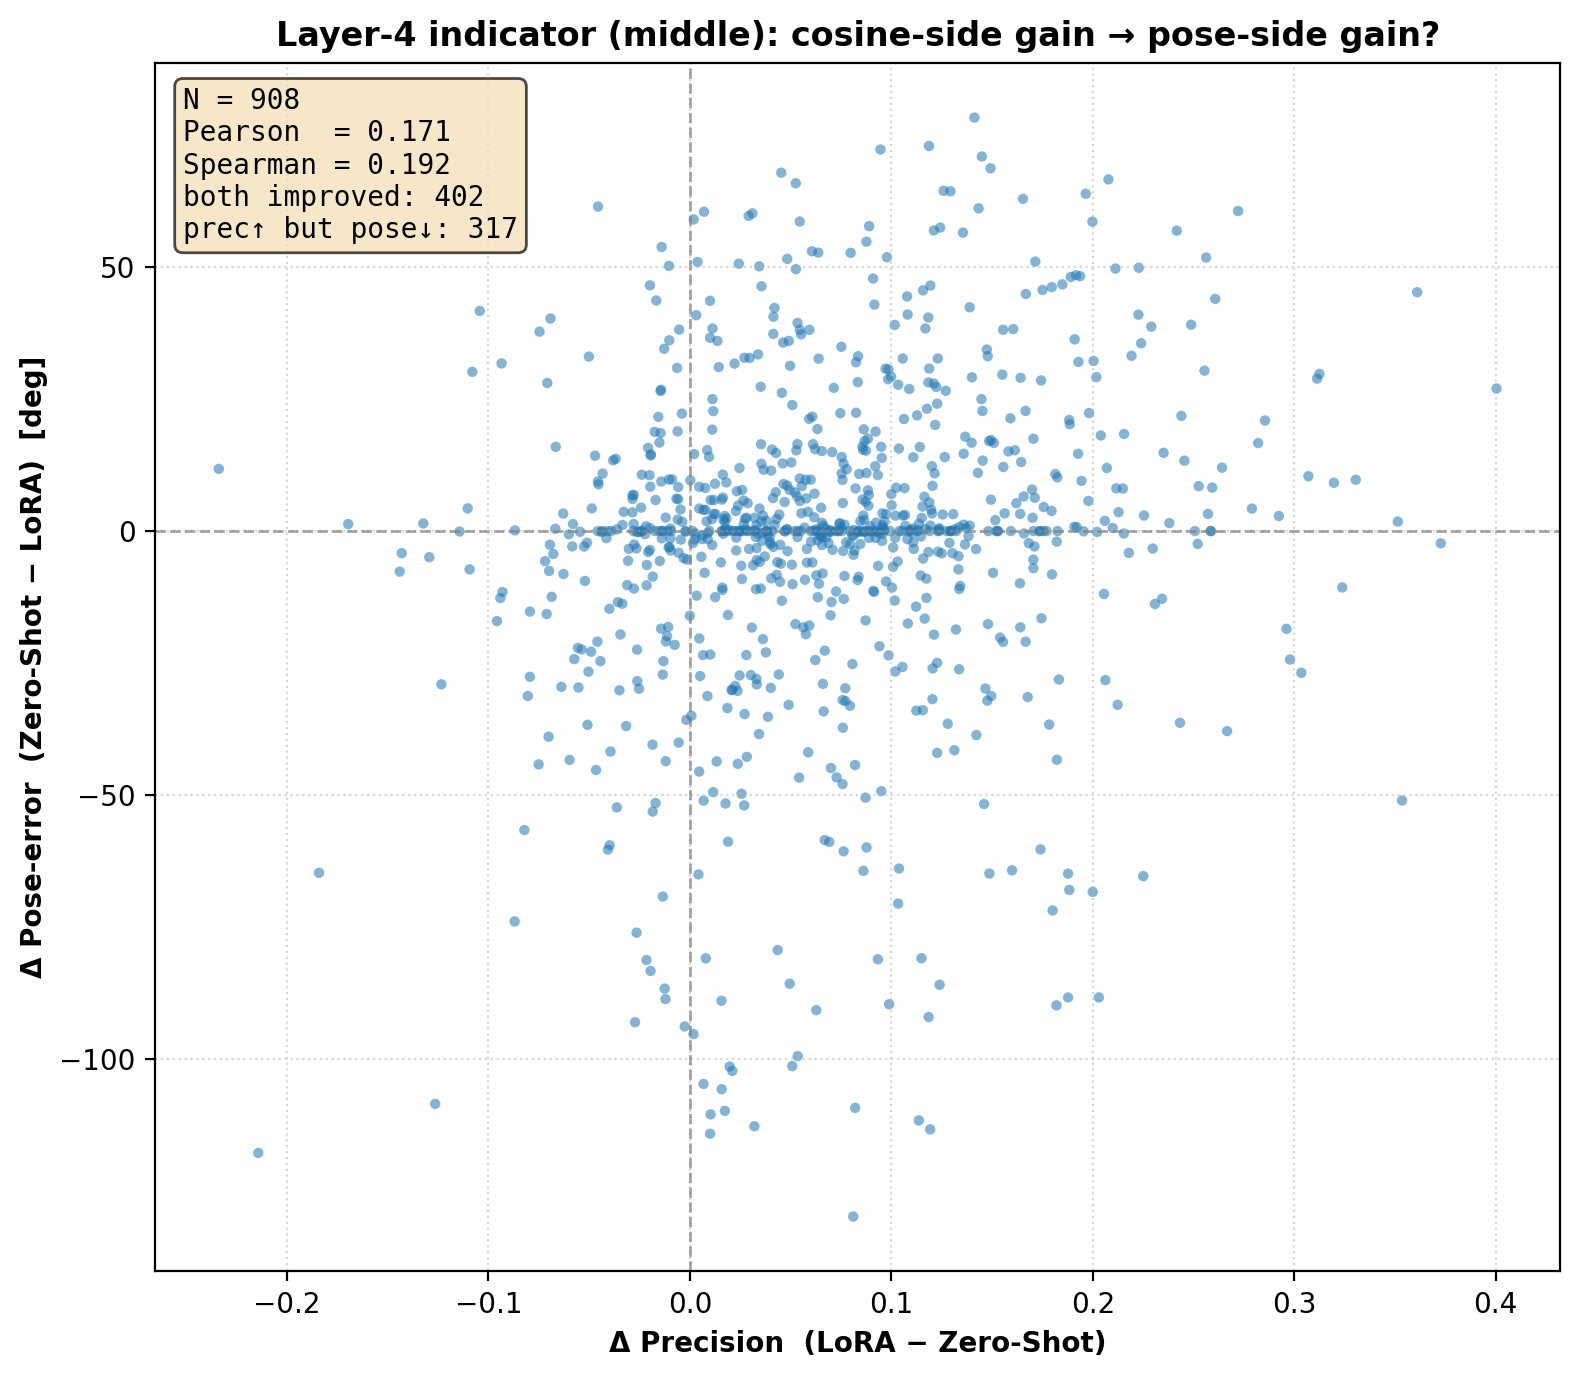
\includegraphics[width=\linewidth]{presentation/result/diag_middle/layer4_scatter_middle.png}
\caption{Pose angle vs.\ Layer-4 cosine}
\label{fig:layer4_scatter}
\end{subfigure}\hfill
\begin{subfigure}{0.42\linewidth}
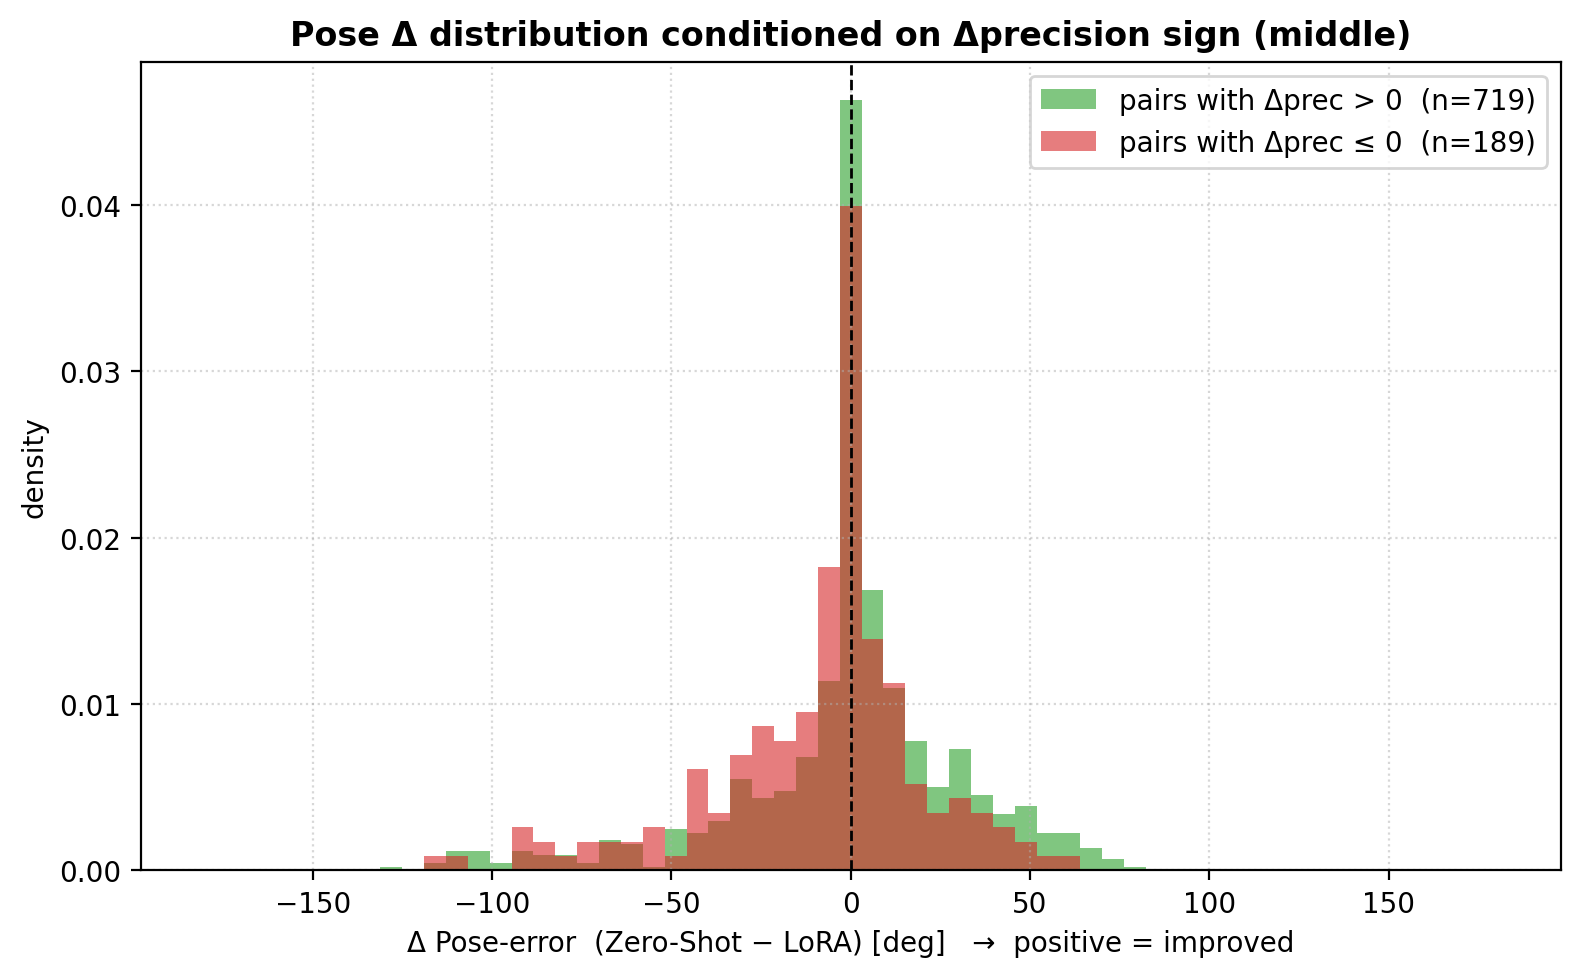
\includegraphics[width=\linewidth]{presentation/result/diag_middle/layer4_pose_hist_middle.png}
\caption{Per-bin Layer-4 cosine histogram}
\label{fig:layer4_pose}
\end{subfigure}
\caption{Layer-4 probe on ViT-L/16. The relationship between camera-pose angle and Layer-4 cosine is
weak, consistent with the global picture that LoRA acts as a small projective tilt on top of
frozen DINOv3 features rather than a re-organisation of intermediate representations.}
\label{fig:layer4}
\end{figure}

Taken together, the diagnostics paint a consistent picture: the NAVI matching gain is real and
reproducible, but it does \emph{not} come from a redesigned feature space. LoRA introduces a small,
low-rank rotation of the existing DINOv3 features that happens to be aligned with NAVI's matching
decision boundary; the underlying representation is essentially unchanged.

\subsection{Limitations and Honest Appraisal}
\label{sec:limits}

We summarise the shortcomings of the present recipe so that they are not misread as features:

\begin{itemize}
    \item \textbf{Strict-threshold pose accuracy does not improve.} AUC@5 is $0.000$ for the
    best-epoch S/16 model and within noise for L/16. The recipe trades strictly correct poses for
    looser correct poses; for downstream applications that require few-degree accuracy this is not
    yet a useful improvement.
    \item \textbf{The feature space barely moves.} Mean intra-image cosine, positive-pair cosine,
    effective rank, neighbourhood dominance, and PCA visualisations all change by $\le 0.02$ in
    absolute terms. This means our recipe is \emph{not} a representation-level fine-tune; it is a
    small projective adjustment on top of frozen DINOv3.
    \item \textbf{Layer-wise behaviour is not pose-disentangled.} The Layer-4 probe shows only a weak
    relationship between camera pose and feature similarity, suggesting that LoRA on Q/V at every
    block does not selectively reshape the layers most relevant to geometry.
    \item \textbf{NAVI is a single-object dataset.} Whether these gains generalise to multi-object
    scenes (MegaDepth, ScanNet, IMC-2021) is untested.
    \item \textbf{No comparison to specialised matchers.} We do not compare against SuperPoint /
    LoFTR / DINOv2-LoRA-with-decoder; the contribution here is bounded to ``zero-shot DINOv3 vs.
    LoRA-tuned DINOv3''.
\end{itemize}

\subsection{Discussion}

Three properties of the recipe are jointly responsible for the (modest) gains:

\begin{enumerate}
    \item \textbf{Zero-init LoRA.} Because $B = 0$ at step~0, the optimizer starts from exactly the
    zero-shot output; the contrastive loss can therefore only \emph{add} information rather than first
    having to recover it from a randomly-initialized projection.
    \item \textbf{True cross-image negatives.} \texttt{batch\_size}\,$=$\,8 means InfoNCE's $K = 128$
    negatives come from seven different scenes, which prevents the loss from collapsing to the
    intra-image $\ln(K + 1)$ trivial floor.
    \item \textbf{Safe Radius.} The 5-patch mask removes spatially adjacent ``negatives'' that share
    physical surface with the anchor; without it the loss is pushed against DINOv3's own local
    smoothness prior and degrades performance instead of improving it.
\end{enumerate}

The two backbones behave qualitatively the same: per-epoch curves are smooth and monotone, and final
gains are within one percentage point of each other (Precision $+7.7$ pp for S/16 vs.\ $+7.0$ pp for
L/16). The smaller absolute Precision of L/16 at zero-shot ($16.8\%$ vs.\ S/16's $17.4\%$) is a known
artefact of the higher feature dimensionality interacting with NAVI's evaluation geometry; the
fine-tuned models close this gap on AUC@20 in favour of L/16 ($1.123$ vs.\ $1.040$).

% ═══════════════════════════════ 5. CONCLUSION ═══════════════════
\section{Conclusion}

We presented a parameter-efficient fine-tuning recipe for DINOv3 dense features that is small in code
(LoRA on Q/V, HardInfoNCE, a 5-patch Safe-Radius mask), small in trainable parameters (rank-4 LoRA
adapters), and small in compute (15 epochs on NAVI). On both ViT-S/16 and ViT-L/16 it improves NAVI
matching Precision by roughly $+7$ percentage points and more than doubles AUC@20 over the zero-shot
baseline. The improvements are reproducible across the two backbone sizes and stable across saved
epochs, suggesting that the gains stem from the recipe rather than from a particular checkpoint or
backbone configuration.

At the same time, the diagnostic analysis (\S\ref{sec:diag}) and the explicit
limitations list (\S\ref{sec:limits}) make clear what this recipe is \emph{not}: it does not reshape
the DINOv3 feature space (intra-image, positive-pair, effective-rank, and PCA diagnostics all move by
$\le 0.02$); it does not improve strict-threshold pose accuracy (AUC@5 stays flat or drops); and it has
only been validated on a single-object dataset. The honest reading is therefore that LoRA + HardInfoNCE
+ Safe Radius applies a \emph{small low-rank tilt} to frozen DINOv3 features that is well-aligned with
NAVI's matching decision boundary, but is far from a full geometric fine-tune. Closing the AUC@5 gap
plausibly requires either training on multi-scene data with explicit hard-negative mining across
scenes, or a stronger adapter family (e.g.\ joint LoRA on Q/K/V plus the FFN), both of which we leave
to future work.

% ═══════════════════════════════ REFERENCES ═══════════════════════
\newpage
\printbibliography[heading=bibintoc,title={References}]

\end{document}
